\section{Exp3: Pushing task in simulation}
The next task was to push a square cube into some target position using
the real robot arm, however preliminary experiments using NAF did not
converge to an intuitively good policy. Instead of rejecting the capabilities
of the NAF algorithm at this stage, simulation experiments was first done in
an ideally setup environment.

\subsection{Environment}

\subsection{Algorithms}

\subsection{Results}

\begin{figure}[h!]
    \centering
    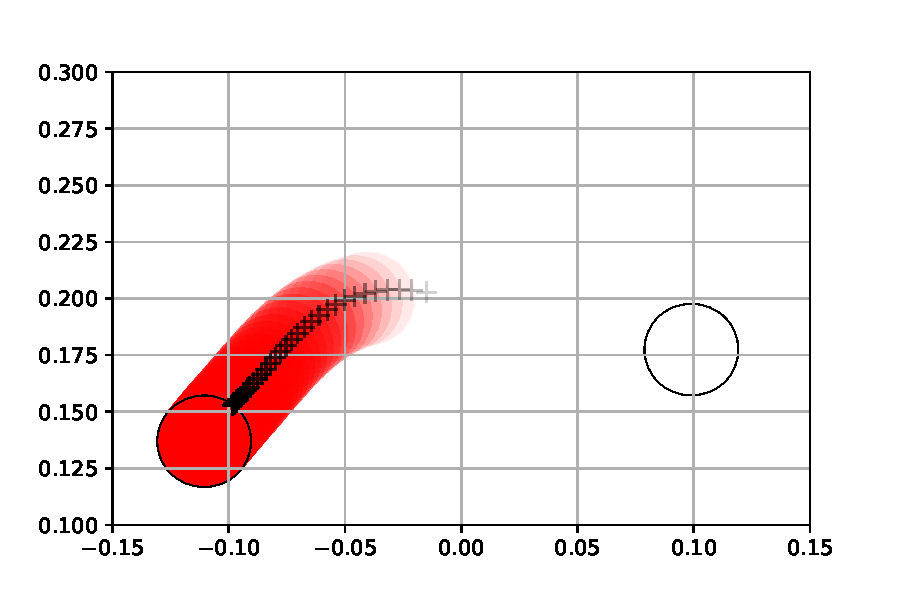
\includegraphics[width=0.4 \textwidth]{res/naf_sim_failure_mode.pdf}
    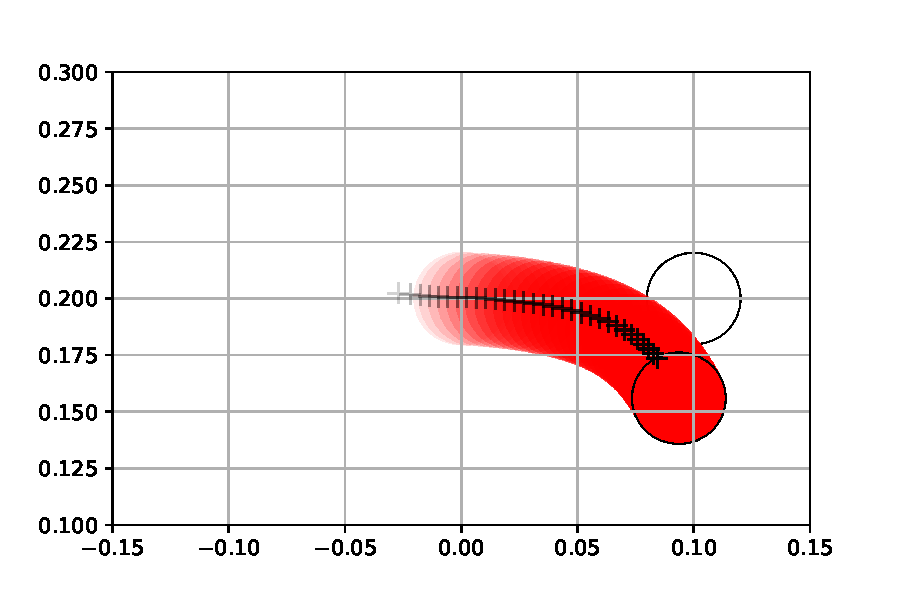
\includegraphics[width=0.4 \textwidth]{res/naf_sim_failure_mode_ideal.pdf}

    \caption{Results of NAF in simulation on pushing task. The red circle is
    the object being pushed, the white circle is the goal, and the cross is the
    simulated end-effector.}

    \label{fig:naf_sim_failure}
\end{figure}

\begin{figure}[h!]
    \centering
    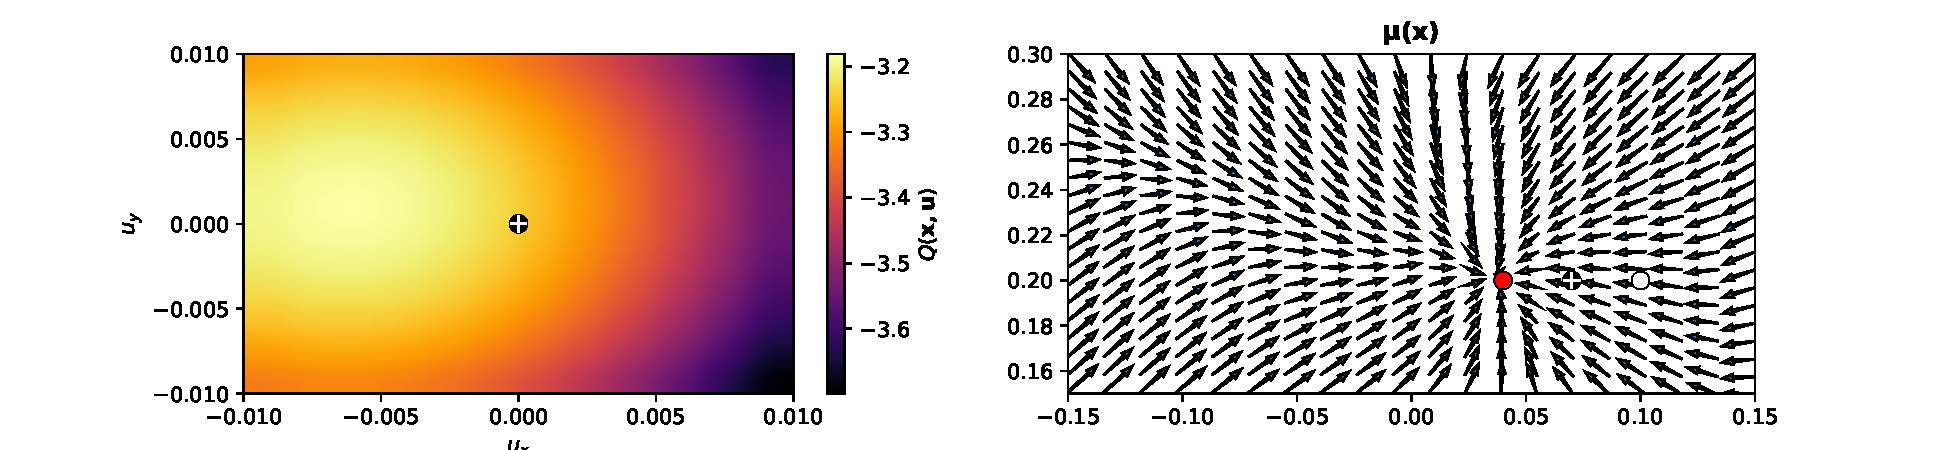
\includegraphics[width=1.0 \textwidth]{res/naf_sim_unimode_q.pdf}

    \caption{Results from using NAF on a simulated pushing task. Q-function and
    policy of the state given by the pushable object (red), the goal (white
    circle), and the end-effector (white cross). Since the advantage function
    is parameterized by a quadratic expression, which is uni-modal, the
    Q-function cannot place more mass on actions corresponding to going up and
    down rather than some intermediate point, and instead in this case the mean
    is placed straight to the left.}

    \label{fig:naf_sim_unimode_q}
\end{figure}
